\chapter{Introdução}

O presente trabalho tem por objetivo apresentar os resultados e conclusões referentes ao projeto final da disciplina Identificação de Sistemas.

O trabalho consiste na análise de um sistema através do projeto de um filtro adaptativo FIR. O sistema utilizado é mostrado na \cref{fig:sistema}. 

\begin{figure}[!h]
	\centering
	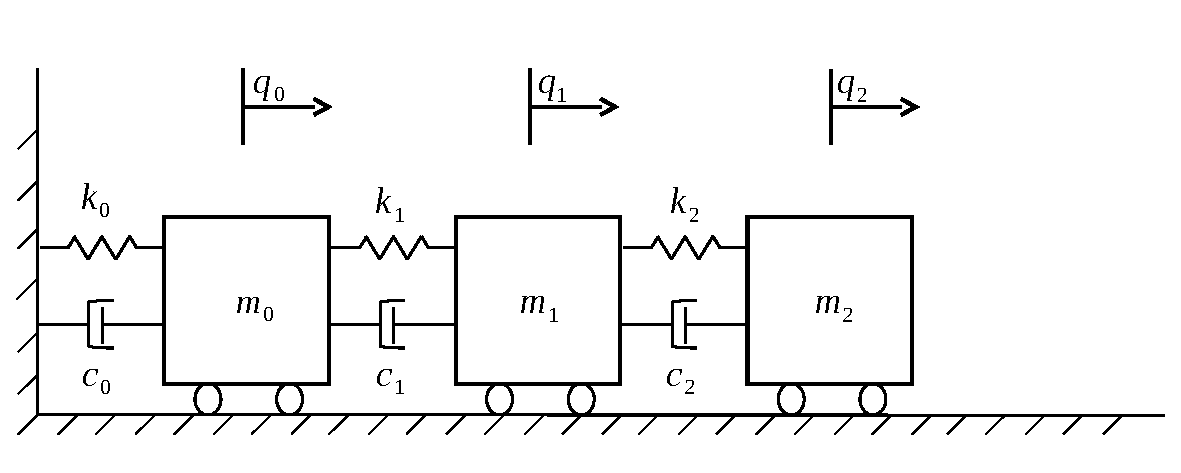
\includegraphics[width=0.8\textwidth]{IMGS/sistema.pdf}
	\caption{Sistema utilizado na análise.}
	\label{fig:sistema}
\end{figure}

\begin{minted}{python}
class A():
	def __init__(self):
		pass
\end{minted}

Do mesmo modo, é imprescindível definir os símbolos, tal como o
conjunto dos números reais $\mathbb{R}$ e o conjunto vazio $\emptyset$.
\symbl{$\mathbb{R}$}{Conjunto dos n\'umeros reais} empty 
\symbl{$\emptyset$}{Conjunto vazio}		


\section{test}
\subsection{teste}